\documentclass[a4paper,11pt]{article}
% Use ctrl + alt + V to view live pdf

% Packages
\usepackage[utf8]{inputenc} % For encoding
\usepackage[T1]{fontenc} % Better handling of accented characters and hyphenation
\usepackage{microtype} % Improves spacing and justification
\usepackage{amsmath, amssymb} % For equations and symbols
\usepackage{graphicx} % For including graphics/images
\usepackage{caption} % For customizing figure and table captions
\usepackage{subcaption} % For subfigures and subcaptions
\usepackage{float} % For fixing figure and table positions
\usepackage{booktabs} % For professional-looking tables
\usepackage{siunitx} % For consistent typesetting of units and numbers
\usepackage[margin=2cm]{geometry} % Adjusts page margins
\usepackage{fancyhdr} % For custom headers and footers
\usepackage{lmodern} % For a professional-looking font (main body font)
\usepackage{titlesec} % For title customization
\usepackage{array} % For custom table formatting
\usepackage[colorlinks=true, linkcolor=black, urlcolor=black]{hyperref} % Colored links without boxes
\usepackage{cleveref} % For improved cross-referencing    
\usepackage{multirow}
\usepackage{enumitem}
\usepackage{listings}
\usepackage{xcolor}
\usepackage{textcomp}
\usepackage{tabularx}
\usepackage{changepage}
\usepackage{tikz}
\usepackage{pdfpages}
\usepackage[table]{xcolor}
\usetikzlibrary{shapes.geometric, arrows}
% --- C++ Style ---
\lstdefinestyle{cpp-style}{
    language=C++,
    basicstyle=\ttfamily\footnotesize,
    keywordstyle=\color{blue}\bfseries,
    stringstyle=\color{orange},
    commentstyle=\color{gray}\itshape,
    numbers=left,
    numberstyle=\tiny\color{gray},
    numbersep=10pt,
    backgroundcolor=\color{white},
    showspaces=false,
    showstringspaces=false,
    breaklines=true,
    breakatwhitespace=true,
    tabsize=4,
    captionpos=b,
    frame=single,
    rulecolor=\color{black},
}

% --- Python Style ---
\lstdefinestyle{python-style}{
    language=Python,
    basicstyle=\ttfamily\footnotesize,
    keywordstyle=\color{blue}\bfseries,
    commentstyle=\color{gray}\itshape,
    stringstyle=\color{green!50!black},
    frame=single,
    breaklines=true,
    showstringspaces=false,
    captionpos=b
}
\renewcommand{\lstlistingname}{Code}
% Custom settings
\pagestyle{fancy}
\fancyhf{}
\fancyhead[L]{\textit{SF4 - DataLogger}} % Header left
\fancyhead[R]{\textit{Will Hewes - wh365}} % Header right 
\fancyfoot[C]{\thepage} % Footer center
\setlength{\headheight}{15pt} % Header height
\setlength{\parindent}{0em} % Indentation for paragraphs
\setlength{\parskip}{0.5em} % Add spacing between paragraphs
\setlength{\abovedisplayskip}{1em}
\setlength{\belowdisplayskip}{1em}
\setlength{\abovedisplayshortskip}{1em}
\setlength{\belowdisplayshortskip}{1em}
% \setlist{topsep=0.2em, partopsep=0em, itemsep=0.1em, parsep=0em}

\graphicspath{{Images/}}

% \renewcommand{\arraystretch}{1.2}

% Title formatting
\renewcommand{\maketitle}{
    \begin{center}
        \LARGE \textbf{ENGINEERING TRIPOS PART IIA} \\[0.5em]
        \Large \textbf{SF4 - DataLogger} \\[0.5em]
        \textbf{Final Report} \\[1.5em]
        \vspace{-1em}
        \small Will Hewes - wh365 \\ 
        Pembroke College \\ 
        \vspace{0.5em}
    \end{center}
}

\begin{document}
\pagenumbering{gobble}
% 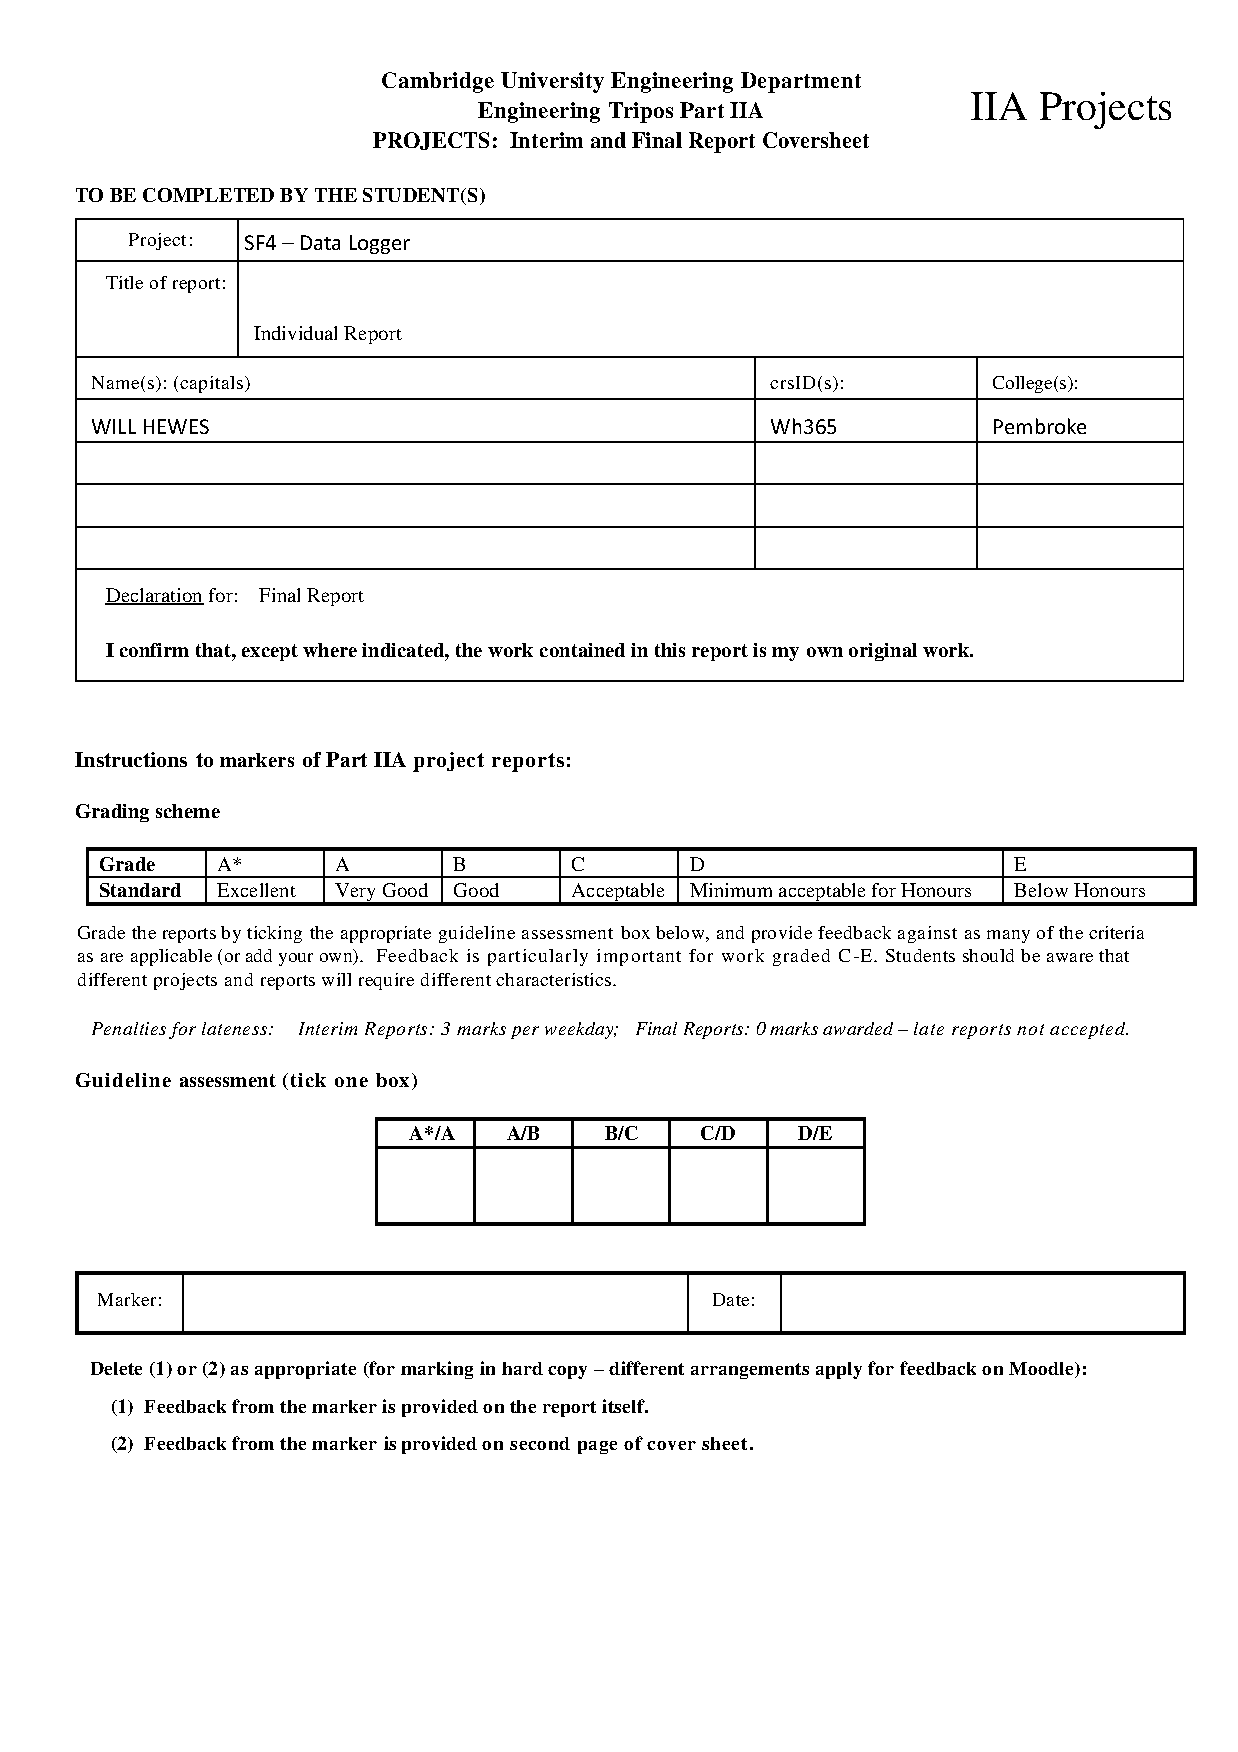
\includepdf[pages=-]{Handouts/IIA_Project_Coversheet Final Report.pdf}
\maketitle
\hrule
\tableofcontents
\newpage
\pagenumbering{arabic} \setcounter{page}{1}

\section{Introduction}
\label{sec:Introduction}

The aim of this project was to develop a microcontroller-based 
automatic plant watering system.
The system can autonomously monitor soil moisture levels, 
plot the data over time, and provide options to water the plant
manually when required or in response to threshold moisture levels.
This allows for effective monitoring and care with minimal user intervention.

In addition to moisture sensing, the system also tracks temperature, 
and was supposed to track humidity and light -
though this could not be implemented due to component delays.
This means most of the key factors affecting plant health
can be closely tracked, enabling detailed analysis of
optimum conditions for plant health.
These additional features enhance the system's utility
for control and research.

The motivation behind creating this autonomous watering system was twofold. 
Firstly, it can be used as demonstrated on a small scale,
allowing direct control over the conditions of one 
or a small number of houseplants,
offering a convenient way to care for plants.
This will remove the majority of the care required
to look after these often frail plants,
which is particularly useful over holidays or 
during the hot Summer months.
As a university student with several well-loved plants,
this has immediate personal appeal.

On a larger scale, the system provides a modular, 
low-cost framework adaptable to industrial or agricultural applications, 
where automated irrigation and environmental monitoring are increasingly valuable.
The low cost and simple design of the system will be appealing 
to large scale, versatile integration,
and the ease with which components can be added
and the GUI customised will allow for rapid expansion into the sector.

\section{Summary}
\label{sec:Summary}
% Summary of overall design decisions and outline of project management (1 side, possible team material)
This section will detail
an outline of the overall project and the decisions taken
to ensure an effective development and deployment.

\subsection{System Functionality}
\label{sec:System_Functionality}

The system developed in this project provides a robust 
and modular platform for automated plant care, 
centred around real-time environmental monitoring and active water delivery. 
It measures soil moisture and ambient temperature via analogue sensors 
connected to a microcontroller, and transmits this information via 
serial connection to a PC for logging and visualisation. 
In response to the measured conditions, 
or through direct user intervention, the system can 
actuate a servo-driven pinch valve that delivers 
a controlled quantity of water from an attached reservoir.

Operation can be either automatic -
based on configurable moisture thresholds -
or manual, with the user issuing commands through a graphical user interface (GUI). 
Sensor data is plotted in real-time and stored in a CSV file,
which will be automatically cleaned after use. 
The complete feedback loop between sensing, user interaction, 
and actuation allows for precise, low-effort maintenance of plant health.

The system was designed to remain extensible beyond its initial demonstration, 
with both the software and hardware structured to accommodate 
additional environmental sensors, remote communication protocols, 
and more sophisticated control schemes.

\subsection{Project Management}
\label{sec:PM}

The project was developed collaboratively in a two-person team, 
with both members working on the system holistically,
applying changes to each module incrementally
as the product was slowly developed.
This approach was taken as opposed to a divided approach,
wherein each member would manage either software or firmware,
with the intention of giving each of us a better understanding 
and overview of the system as a whole,
allowing both of us to effectively contribute ideas 
concerning the whole project collaboratively. 
This had the consequence that on occasion we would 
both be making changes to the same module simultaneously.

By nature of this development style,
there was an increased risk of conflicts introduced to the system
if we did not take proper care to ensure that our changes were compatable.
As a result, version control and clear communication 
became a vital aspect of our project management.

Version control and collaborative development were managed using GitHub, 
enabling parallel work on the codebase
and simplifying the process of merging changes and tracking development history. 
This also allowed modular elements - 
such as the GUI framework and firmware routines -
to be developed and tested in isolation before being brought together.

The project followed a phased development structure:
\begin{enumerate}[nosep]
    \item \textbf{Component Validation:} 
    Initial sessions focused on validating the individual sensors 
    and actuators through breadboard testing, 
    ensuring reliable signal acquisition and control.
    \item \textbf{Prototype Development:} 
    In parallel with circuit construction, a socket-based simulation 
    of the Arduino-PC interface was created to support 
    early development of the GUI and data parsing routines 
    in the absence of hardware.
    \item \textbf{System Integration and Testing:} 
    Once physical components were functional, development transitioned 
    to serial communication over USB. 
    Modules were progressively integrated and tested together 
    in a final working system.
\end{enumerate}

Throughout the project, care was taken to adopt a modular workflow, 
with each subcomponent independently tested and versioned. 
This reduced the risk of cascading failures during integration and 
supported incremental development even in the face of hardware delays 
or debugging setbacks.

\subsection{System Architecture}
\label{sec:System_Architecture}

The system architecture was designed around a clear separation 
of responsibilities between the microcontroller and the host PC, 
with a serial communication link serving as the bridge. 
This enabled a modular division of tasks, simplified debugging, 
and ensured that each side of the system could be developed and tested independently.

On the Arduino side, responsibilities included real-time sampling of sensor data, 
basic calibration and averaging of analogue values, 
formatting of output strings for serial transmission, 
and all control logic relating to the servo actuation. 
The microcontroller also responded to incoming configuration commands from the PC, 
such as updating moisture thresholds or toggling the warning indicator.

The PC software, written in Python, handled all higher-level data processing 
and user interaction. 
Upon receiving sensor data over the serial connection, 
it parsed and logged the data to a CSV file 
and plotted the live sensor readings in a responsive GUI. 
This GUI also provided the user with control over watering modes 
and threshold parameters, 
which were sent back to the Arduino for immediate application.

During early development, the communication protocol was prototyped 
using a TCP socket-based simulation of the Arduino output. 
This approach allowed the software framework to be built 
and tested before the hardware was available. 
Once the physical circuit was operational, 
the system transitioned to serial-over-USB 
communication without requiring significant changes to the data handling routines. 
The decision to maintain a consistent communication format 
across these stages proved highly effective and kept integration overhead minimal.

The architecture was deliberately designed with extensibility in mind. 
Additional sensors - digital or analogue — 
can be easily integrated on either side of the interface, 
with the firmware structured to accommodate future expansion. 
Similarly, the current serial protocol could be replaced with 
Bluetooth or Wi-Fi with minimal disruption to the existing software infrastructure, 
enhancing portability and enabling 
remote monitoring or control in future versions of the system.

\subsection{Hardware Selection}
% Sensors and actuators, with brief justification (no electrical detail)

\begin{table}[H]
    \centering
    \renewcommand{\arraystretch}{1.5} 
    \makebox[\linewidth][c]{
    \resizebox{0.8\textwidth}{!}{
    \begin{tabular}{|c|c|c|}
        \hline
        \textbf{Order Code} & \textbf{Description of Component} & \textbf{Unit Price (£)} \\
        \hline
        2946124 & Capacitive Soil Moisture Sensor Module & 4.69 \\
        \hline
        SC21096 & Mini servo & 2.94 \\
        \hline
        4030054 & Temperature sensor & 1.38 \\
        \hline
        \rowcolor{yellow!60} 3167525 & Light sensor & 1.43 \\
        \hline
        \rowcolor{yellow!60} SN36746 & Humidity sensor & 0.91 \\
        \hline
        \multicolumn{2}{|c|}{\textbf{\large Total}} & \textbf{\large 11.35} \\
        \hline
    \end{tabular}
    }   
    }
    \caption{Component Order Summary}
    \label{tab:component_order}
\end{table}

\section{System Architecture}
\label{sec:System_Architecture}
% Include anmalogue circuitry, block diagram, and decision to include capacitors, lack of resistors etc.
% External power supply for servo

- block diagram\\
- description of general structure

\begin{figure}[H]
    \centering
    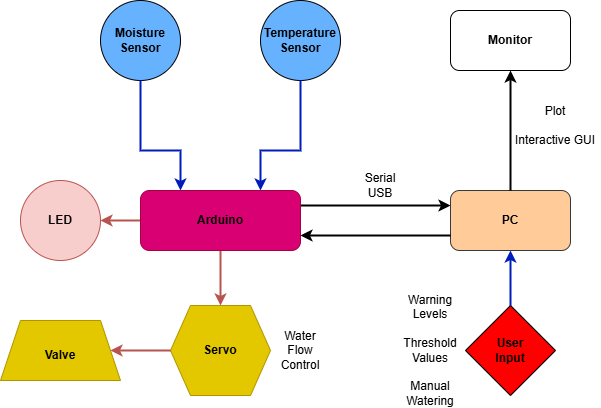
\includegraphics[width=0.8\textwidth]{Datalogger Block Diagram - final.png}
    \caption{Block Diagram for the automatic watering system}
    \label{fig:Block_Diagram_for_the_automatic_watering_system}
\end{figure}

\subsection{Circuit Design}
\label{Cicuit_Design}

- diagram\\
- testing sensors\\
- servo on seperate rail\\ 
- need for capacitors

\begin{figure}[H]
    \centering
    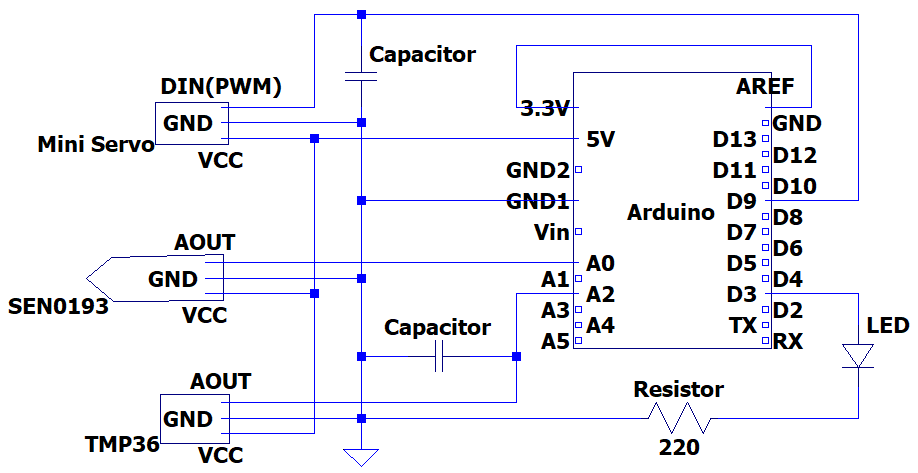
\includegraphics[width=0.8\textwidth]{Analogue Circuit Diagram - final.png}
    \caption{Analogue Circuit Diagram for the automatic watering system}
    \label{fig:Analogue_Circuit_Diagram_for_the_automatic_watering_system}
\end{figure}

\subsection{Watering System}
\label{sec:Watering_System}

- decision to use pinch valve\\
- necessity of reservoir sensor\\ 
- demonstration of components individually and collectively

\section{Code}
\label{sec:Code}
% Description of design/ computer code
\subsection{Firmware}
\label{sec:Firmware}
- sensors\\
- parsing, processing\\
- servo control

\subsection{Software}
\label{sec:Software}
- comms with Arduino\\
- GUI, plotting\\
- initial demonstration

\section{Technical Problemms}
\label{sec:Technical_Problems}
% Outline problems encountered in development and their technical solutions
- get Chengs help in drafting some interesting ones \\
- outline problem with powerrail if appropriate (not realising that these breadboards come with a gap in the powerrail)\\
- floating point problem for temp sensor

\section{Test Procedure}
\label{sec:Test_Procedure}
% Test procedure and software implementation
- testing individual compomnents one at a time \\
- testing the software presentation with a demonstration random data supply\\
- calibrating the moisture sensor with dry and with water\\
- determining the required servo rotation to elicit small quanmtiy of water\\
- use data from other sources to determine if humidity, light, and temp calibrated properly

\section{Further Improvements}
\label{sec:Further_Improvements}
- wifi module \\
- less jerryrigged water supply\\
- more sensors (CO2 conc)\\
- reservoir sensor\\
- greater control over parameters (mass of plant, type of plant)\\
- greater signal processing\\
- wider industrial applications

\subsection{Wider Industry}
\label{sec:Wider_Industry}
% Mention the watering systems currently being developed and the research undertaken
- deeper research into exact requirements\\
- close collaboration with farmers to set these requirements\\
- integrate a warning system to say that the specific conditions have been met (humidity requirements for harvesting etc, perhaps dangerous levels of heat)\\
- further integration of sensors, such as soil content (salt conc, fertiliser etc.)

\section{Conclusion}
\label{sec:Conclusion}

The aim of this project was to create a working demonstration of 
our autonomous watering system, with the ability to both log data
and dispense controlled quantities of water 
as the consumer dictates.
Overall, this has been a resounding success, 
acheiving the inital goal of moisture sensing and servo activation,
and expanding on this to include other senors 
and a more developed GUI.

The primary challenges and takeaways for a similar project in the future
include ...
Throughout this report it is evident that responsible practises 
such as detailed planning, modular testing,
and a feasible but expandable scope are integral to 
ensuring the success of a project like this.

This work could be expanded in the future to make a 
more sophisticated and professional datalogger
of the same scale,
incorporating more sensors, a more ... housing and 
general setup,
or could be further modified to be used in larger
industrial applications, such as informing agricultural farming
as is being researched by ...

\newpage
\appendix
\begin{thebibliography}{9}

\bibitem{arduino_servo}
Arduino. \textit{Servo Motor Basics with Arduino} : \\
\url{https://docs.arduino.cc/learn/electronics/servo-motors/}

\bibitem{tmp36}
Analog Devices. \textit{TMP35/TMP36/TMP37 Data Sheet} : \\
\url{https://www.analog.com/en/products/tmp36.html} 

\bibitem{arduino_tmp36}
ArduinoGetStarted. \textit{Arduino - TMP36 Temperature Sensor} : \\
\url{https://arduinogetstarted.com/tutorials/arduino-tmp36-temperature-sensor}

\bibitem{dfrobot}
DFRobot. \textit{Capacitive Soil Moisture Sensor SKU SEN0193} : \\
\url{https://wiki.dfrobot.com/Capacitive_Soil_Moisture_Sensor_SKU_SEN0193}

\bibitem{pinch_valve_design}
Printables. \textit{Pinch Valve Powered by Servo} : \\
\url{https://www.printables.com/model/247744-pinch-valve-powered-by-servo/files}

\end{thebibliography}

\section{Interim Report}
% 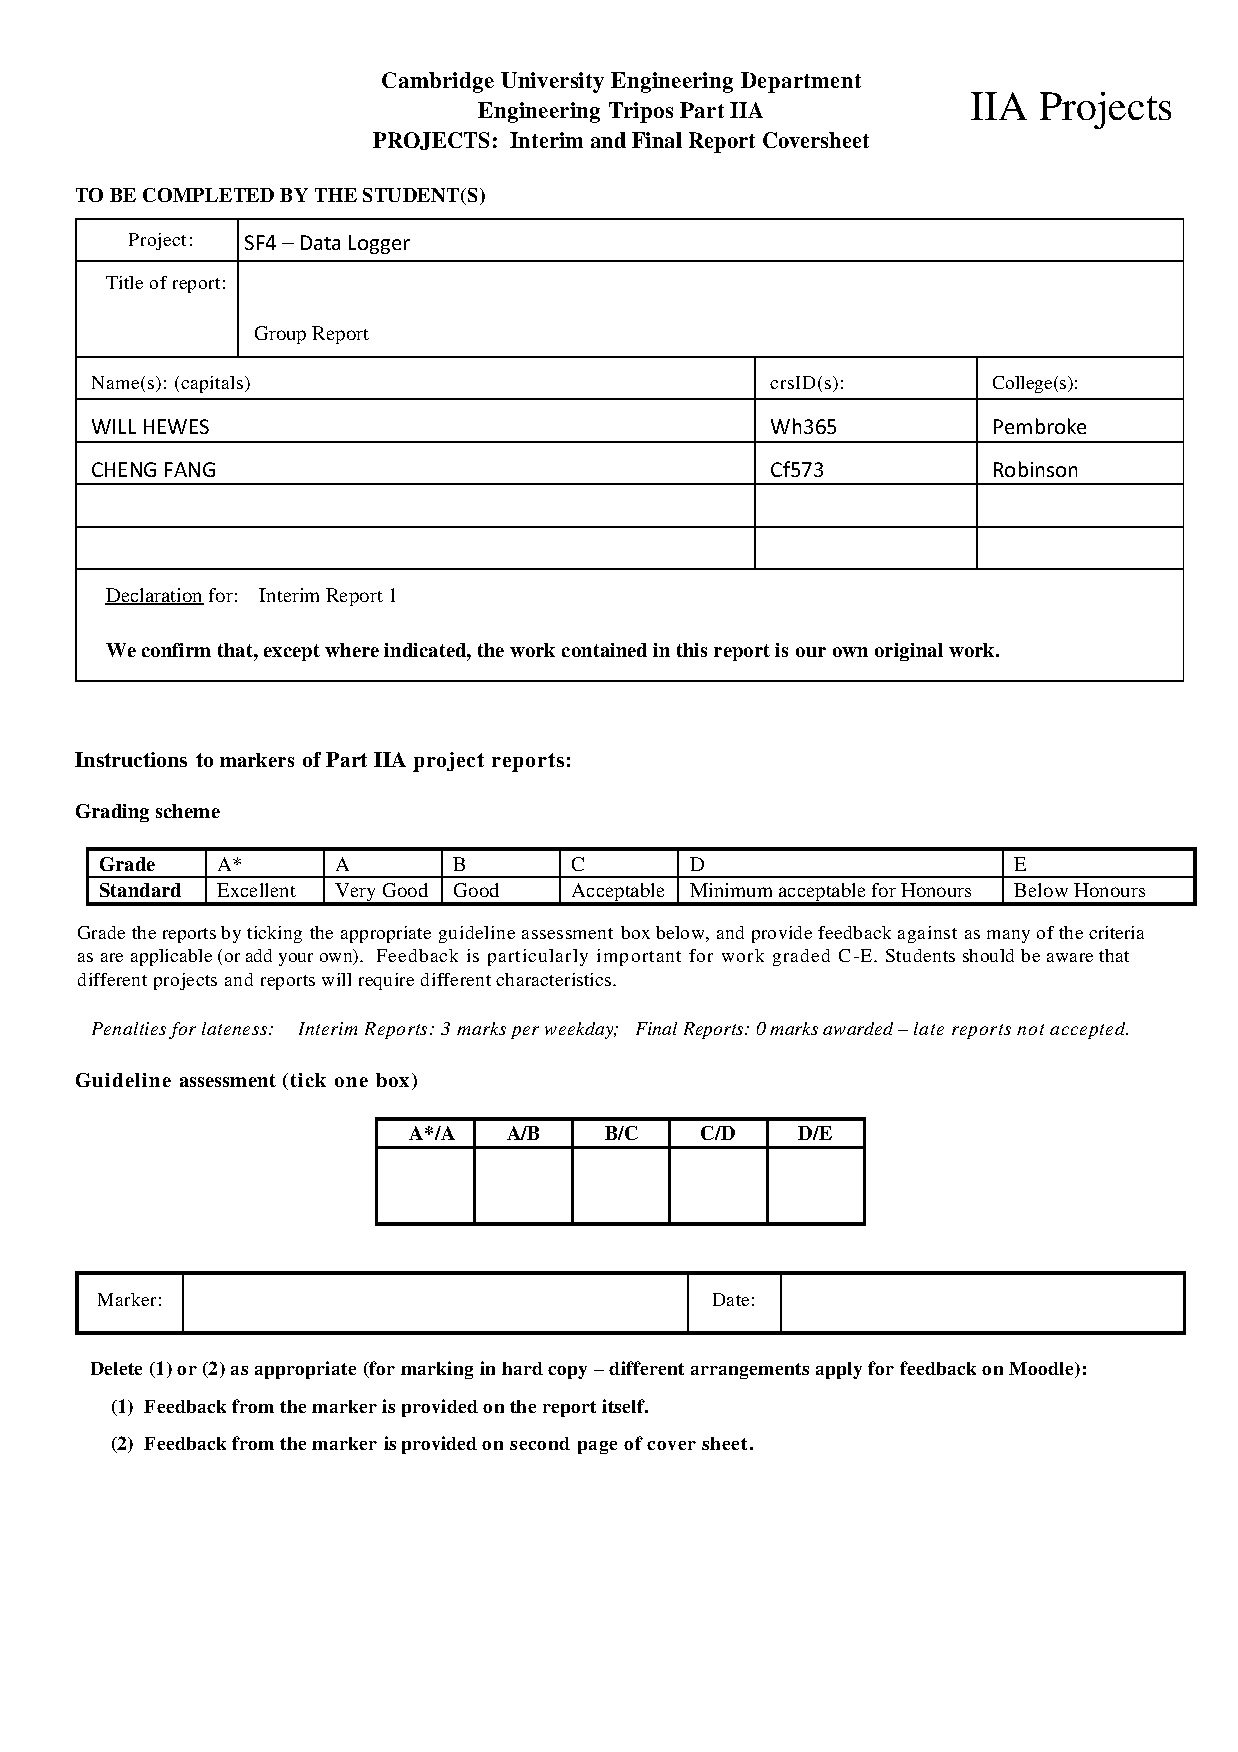
\includepdf[pages=-]{Reports/First Interim Report.pdf} % e.g. [pages={1,3-5,7}] to include pages 1,3,4,5,7
% Featuring the Interim Report

\end{document}